Two banana  plugs $X_{6A}$ and $X_{6B}$  provide the connection to  the output
voltage, while reverse voltage protection is achieved via diode $V_4$.

\begin{figure}[th!]
    \center
    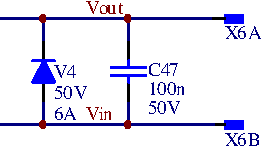
\includegraphics[width=.35\textwidth]{images/circuit/output-connectors.pdf}
    \caption{reverse voltage protection at output}
    \label{fig:circuit:output}
\end{figure}

An external  reference voltage of \SI{1.5}{\volt}  is used to ensure  that the
ADCs and DACs can  make accurate measurements and can be  used over their full
range (see figure \ref{fig:circuit:vref}).

\begin{figure}[th!]
    \center
    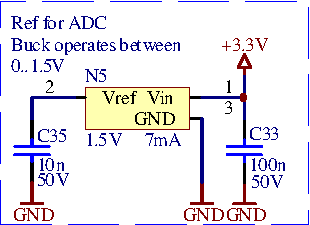
\includegraphics[width=.4\textwidth]{images/circuit/vref.pdf}
    \caption{%
        \SI{1.5}{\volt} reference voltage for full-range operation of DACs and
        DACs
    }
    \label{fig:circuit:vref}
\end{figure}
